\section{Results}

\begin {itemize}
% After the previous selection of genes we worked with 191 genes
% decided to choose 5 clusters
\item Spline regression:
 The 2 first clusters included the genes with an L-shape

\begin{center}
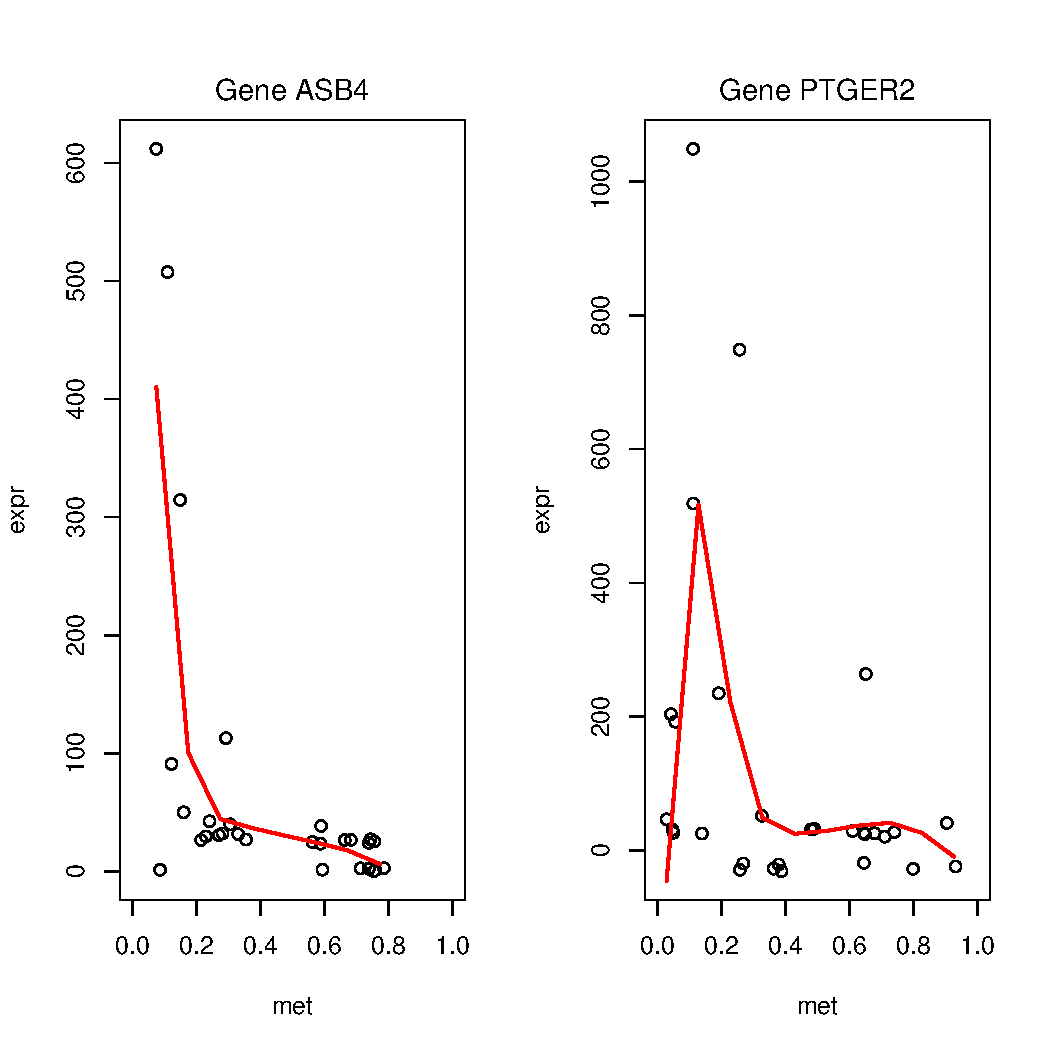
\includegraphics[width=0.3\columnwidth]{./images/grafic_two_patterns.pdf}
\end{center}

\item Conditional Mutual Information

% No previous selection of the genes was needed
%\begin{block}{Three criteria}
We filtered for L-shapes using a combination of three criteria:
\begin{itemize}
\item the ratio $r<0.25$
\item unconditioned MI $\mathit{cMI}(0)>0.1$
\item the median expression on the left side of the optimal threshold $t^{\ast}$ is higher
than the median expression on the right side.
\end{itemize}
%\end{block}
% The parameters are chosen according to a random permutation test (see Liu(2012)).
% According to the above criteria, a total of 641 genes are selected to be L-shape genes.


\item Comparison between the methods:
\begin{center}
\begin{tabular}{|c|c|c|}
\hline
Initial selection & 191 & 641 \\
\hline
\hline
Cluster & Splines & cMI \\
\hline
1 & 140 & 102 \\
2 & 22 & 16 \\
\hline
Total & 162 & 118 \\
\hline 
\end{tabular}
\end{center}

\item In summary...
  \begin{itemize}
  \item We have found similar results between both methods.
  \item Biological interpretation is in progress but preliminary (unpublished) results are consistent with the hypothesis.
  \item Sample size is a limiting factor: $cMI$ works better with hundreds of samples but one may have a very small number (real cases: 30, 12)
\end{itemize}

%\begin{center}
%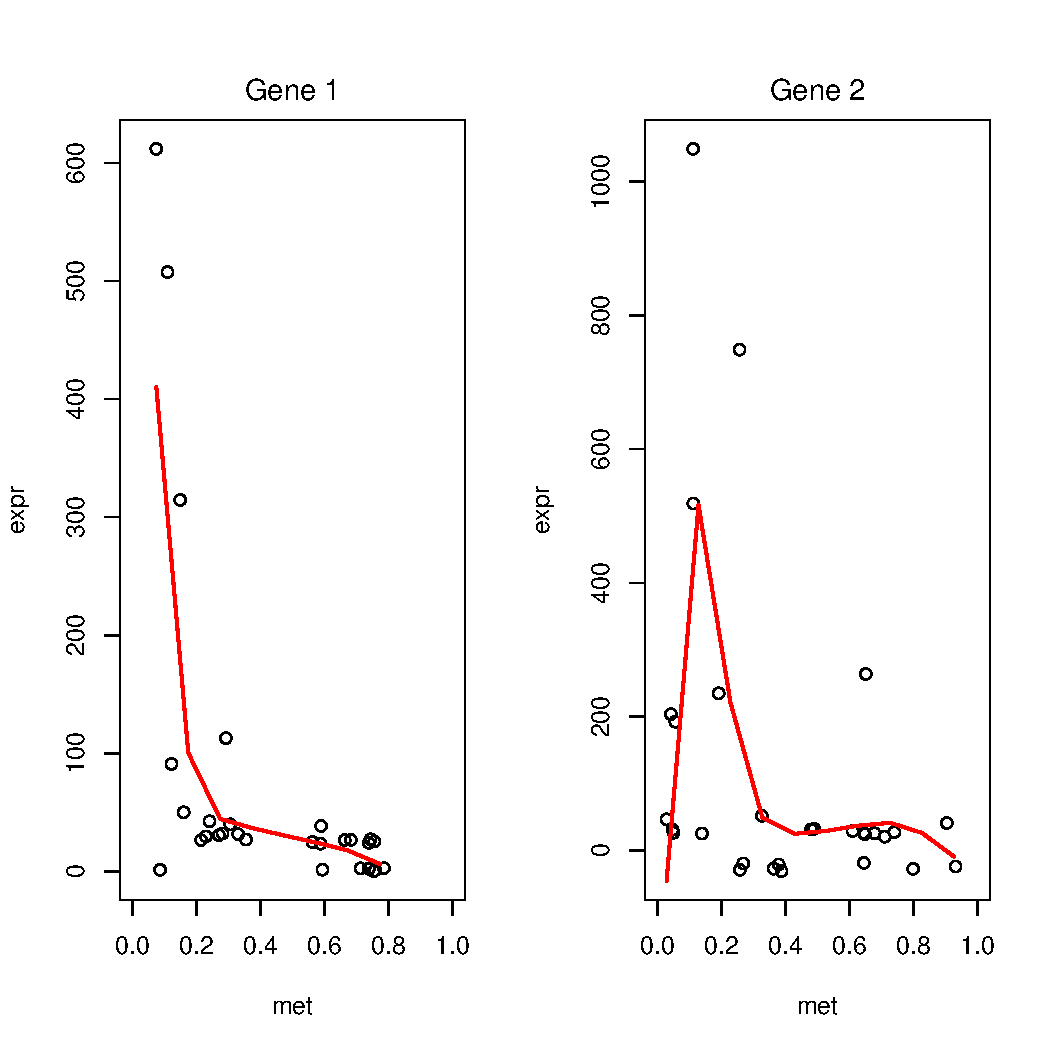
\includegraphics[width=0.6\columnwidth]{./images/grafic_two_genes.pdf}
%\end{center}

\end{itemize}


